\documentclass[12pt]{article}

\usepackage{alphabeta}
\usepackage[greek, english]{babel}
\usepackage[utf8]{inputenc}
\usepackage{geometry}
\usepackage{graphicx}
\usepackage{amsmath}
\usepackage{float}
\usepackage{amsfonts}

\DeclareMathOperator*{\argmax}{arg\,max}

\graphicspath{{images/}}
\geometry{left=.3in, right=.3in, top=0.6in, bottom=0.6in}
\renewcommand{\baselinestretch}{1.2}
\pagenumbering{gobble}
\let\endtitlepage\relax

\begin{document}
%% -------------------------------------------------------------------------------------
    \begin{titlepage}
    \vspace*{-0.6in}
    \begin{flushleft}
        
\includegraphics[scale=0.44]{images/logo.png}
        
        \vspace{1cm}
        \textbf{Ονοματεπώνυμο:} Ανδρέας Γουλέτας (3170031), Λούντζης Λάμπρος (3170095)\\ 
        \textbf{Εργασία:} Τεχνητή Νοημοσύνη\\
        \textbf{Ημερομηνία:} 20 Ιανουαρίου 2021
        
    \end{flushleft}
    \vspace{0.2in}
\end{titlepage}
    
%% -------------------------------------------------------------------------------------
\section{Εισαγωγή}
\subsection{Περιγραφή Εργασίας}
Δοθέντος του συνόλου δεδομένων \textbf{IMDb Dataset}, καλούμαστε να εκπαιδεύσουμε δύο μοντέλα μηχανικής μάθησης με σκοπό την \textbf{κατάταξη (classification)} κριτικών ταινιών σε δυο κατηγορίες, θετικές και ανρητικές.\\\\
Για την λύση του προβλήματος της κατάταξης, επιλέξαμε τους αλγορίθμους επιβλεπόμενης μάθησης \textbf{Multinomial Naive Bayes} και \textbf{Random Forest} με χρήση \textbf{ID3} δέντρων. Οι αλγόριθμοι εκπαιδεύονται στο 90\% των δεδομένων του συνόλου εκπαίδευσης του IMDb Dataset, οι υπερπαράμετροί τους επιλέγονται με την την χρήση του υπόλοιπου 10\% του συνόλου εκπαίδευσης, ως δεδομένα επικύρωσης, και τέλος αξιολογούνται στα δεδομένα του συνόλου αξιολόγησης του IMDb Dataset.

\subsection{Δομή παραδοτέου}
Αρχικά, στην Ενότητα 2 περιγράφεται η επεξεργασία που έχουν υποστεί τα δεδομένα. Στην Ενότητα 3 παρουσιάζεται η μέθοδος της επιλογής χαρακτηριστικών, τα προβλήματα που λύνουμε κάνοντας χρήση της καθώς επίσης και το μοντέλο του κλερδους πληροφορίας. Στην Ενότητα 4 παρουσιάζεται ο ταξινομητής Multinomial Naive Bayes, καθώς και τα αποτελέσματα που δίνει μέσω καμπυλών αξιολόγησης. Τέλος, στην Ενότητα 5 παρουσιάζεται ο ταξινομητής Random Forest με δέντα αποφάσεων ID3 μαζί και τα αποτελέσματά του που έχουμε εξάγει σε καμπύλες αξιολόγησης.

%% -------------------------------------------------------------------------------------
\section{Επεξεργασία Δεδομένων}
Για να χρησιμοποιήσουμε τη συλλογή IMDb Dataset, θα πρέπει τα κείμενα να μετασχηματιστούν με τέτοιο τρόπο ώστε να μπορούν να χρησιμοποιηθούν απο τα μοντέλα μας.\\
Αρχικά, τα κείμενα σπάνε σε όρους (tokenization), οπου κάθε όρος είναι μια λέξη του κείμενου. Έπειτα, γίνεται αφαίρεση σημείων στίξης και άλλων χαρακτήρων που δεν σχηματίζουν ακολουθίες από γράμματα και αριθμούς. Τέλος, κάθε όρος κανονικοποιείται χρησιμοποιώντας case-folding, δηλαδή μετατρέποντάς τον σε πεζά γράμματα.

\subsection{Αφαίρεση stop words}
Παρότι την παραπάνω επεξεργασία, παρατηρούμε ότι υπάρχουν κάποιοι όροι που εμφανίζονται συχνά στα κείμενα οι οποίοι παρέχουν μικρή αξία στην κατάταξη των κειμένων. Χαρακτηριστικά παραδείγματα, είναι οι όροι the, a, an, this κλπ. Αυτοί οι όροι ονομάζονται \textbf{stop words}, και επειδή δεν βοηθούν στην κατάταξη των κειμένων τους αφαιρούμε.\\

\subsection{Stemming}
Mια ακόμα μορφή κανονικοποίησης που χρησιμοποιούμε, για να μειώσουμε το λεξιλόγιό μας, είναι η αποκοπή καταλήξεων με \textbf{stemming}. Σκοπός της τεχνικής αυτής είναι να περικόψει τις κλιτικές καταλήξεις και να ανάγει τις παράγωγες λέξεις σε μια κοινη μορφή, το \textbf{stem}. Την παραπάνω υλοποίηση την επιτυγχάνουμε με την χρήση του \textbf{Porter stemmer}, που είναι ένας αλγοριθμικός stemmer.\\\\
\underline{\textbf{παράδειγμα:}} biology, biological, biologically $\rightarrow$ biolog

\subsection{Vectorization}
Είδικα στο μοντέλο Random Forest, τα κείμενα παίρνουν την μορφή \textbf{διανυσμάτων (vector)}. Τα διανύσματα έχουν μέγεθος ανάλογο του συνόλου των χαρακτηριστικών που χρησιμοποιούνται και κάθε θέση του διανύσματος έχει τιμή 0, άν το χαρακτηριστικό δεν υπάρχει στο κείμενο, ή 1, αν το χαρακτηριστικό υπάρχει.\\\\
\underline{\textbf{παράδειγμα:}} Έστω το κείμενο $d_{1}$ σε διανυσματική μορφή γίνεται: $d_{1}$: $<X_{1}, X_{2}, X_{3} ..., X_{n}>$ = $<1, 0, 0, ..., 1>$ οπου $X_{i}$ είναι ένα χαρακτηριστικο. 

%% -------------------------------------------------------------------------------------
\section{Επιλογή Χαρακτηριστικών}
Οι αλγόριθμοι μηχανικής μάθησης που υλοποιούμε, προκειμένου να κατατάξουν τα κείμενα στην σωστή κατηγορία χρειάζονται ένα σύνολο \textbf{χαρακτηρισιτικών}. Αυτό το σύνολο χαρακτηρισιτκών ταυτίζεται με τις μοναδικές λέξεις που μπορούν να προκείψουν από τα δεδομένα εκπαίδευσης, γνωστό και ως \textbf{λεξιλόγιο (vocabulary)}.\\
Είναι εύλογο να αποφανθούμε οτι λόγω της μεγάλης έκτασης των χαρακτηριστικών, η απόδοση των ταξινομητών μας κατά την εκπαίδευση και την εφαρμογή τους δεν είναι η καλύτερη δυνατή. Εκτός αυτού, υπάρχουν \textbf{χαρακτηριστικά θορύβου (noise features)} τα οποία αυξάνουν το σφάλμα κατάταξης (classification error) σε νέα δεδομένα.\\
Για την επίλυση των παραπάνω προβλημάτων επιλέγουμε ένα υποσύνολο των διαθέσιμων χαρακτηριστικών και συγκεκριμένα αυτών που παρέχουν αρκετή ποσότητα πληροφορίας, ώστε ο αλγόριθμός μας να πάρει την σωστή απόφαση κατάταξης. Η διαδικασία αυτή ονομάζεται \textbf{επιλογή χαρακτηριστικών (feature selection)}. Η η υλοποίησή της βασίζεται στo \textbf{κέρδος πληροφορίας (information gain)}, που δίνεται από την εξίσωση:
\begin{equation*}
    IG(X;C) = H(C) - \sum_{x}^{}P(X=x)*H(C|X=x)
\end{equation*}
όπου $Η(C)$ είναι η εντροπία της κλάσσης C και $H(C|X=x)$ είναι η εντροπία της κλάσσης C αν γνωρίζουμε ότι η τιμή του χαρακτηριστικού Χ είναι x.

%% -------------------------------------------------------------------------------------
\section{Multinomial Naive Bayes}
Το μοντέλο \textbf{multinomial Naive Bayes} αποτελεί μια πιθανοτική μέθοδο επιβλεπόμενης μάθησης. Σκοπός του μοντέλου είναι να βρεί την πιθανότερη κλάση (θετική ή αρνητική κριτική) για κάθε κείμενο:
\begin{equation*}
 c_{map} = \argmax_{c \in \mathbb{C}} P(c|d) = \argmax_{c \in \mathbb{C}} P(c) \prod_{1 \leq k \leq n_{d}}^{}P(t_{k}|c)
\end{equation*}
όπου $P(t_{k}|c)$ είναι η δεσμευμένη πιθανότητα ενός όρου $t_{k}$ να βρίσκεται σε ένα κείμενο της κλάσης c και $P(c)$ είναι η a priori πιθανότητα ενός κειμένου να ανήκει στην κλάση c.\\\\
Στην παραπάνω εξίσωση παρατηρούμε ότι γίνεται πολλαπλασιασμός πολλών πιθανοτήτων, με κίνδυνο υποχείλισης. Γι' αυτό, επιλέγουμε να λογαριθμίσουμε την παραπάνω εξίσωση ώστε να έχουμε άθροίσματα πιθανοτήτων:
\begin{equation*}
    c_{map} = \argmax_{c \in \mathbb{C}} ( \log{P(c)} + \sum_{1 \leq k \leq n_{d}}^{}\log{P(t_{k}|c)} )
\end{equation*}\\
Η a priori πιθανότητα δίνεται από την εξίσωση:
\begin{equation*}
    P(c) = \frac{N_{c}}{N}
\end{equation*}
όπου $N_{c}$ είναι ο αριθμός των κειμένων στην κλάση c και $N$ είναι ο συνολικός αριθμός των κείμένων. Αντίστοιχα, η δεσμευμένη πιθανότητα είναι:
\begin{equation*}
    P(t_{k}|c) = \frac{T_{tc} + 1}{\sum_{t' \in V}^{}(T_{t'c}+1)}
\end{equation*}
όπου $T_{tc}$ είναι η \textbf{συχνότητα (term frequency)} του όρου t στα δεδομένα εκπαίδευσης της κλάσης c.\\\\
Η συχνότητα ενός όρου στα κείμενα εκπαίδευσης της κλάσης c έχει ένα μειονέκτημα: όλοι οι όροι θεωρούνται εξίσου σημαντικοί όσο αναφορά την κατάταξη του κειμένου. Γι' αυτό, επιλέγουμε να χρησιμοποιήσουμε την \textbf{συχνότητα κειμένου (document frequency)}, που ορίζεται ως το πλήθος των κειμένων της συλλογής που περιέχουν τον όρο t. Η παραπνάνω εξίσωση μετατρέπεται ως εξης:
\begin{equation*}
    P(t_{k}|c) = \frac{df_{tc} + 1}{\sum_{t' \in V}^{}(df_{t'c}+1)}
\end{equation*}

\subsection{Επιλογή Χαρακτηριστικών}
Όπως αναφέρθηκε στην Ενότητα 3, προκειμένου ο ταξινομητής Naive Bayes να είναι αποδοτικός κατά την εκπαίδευση και την εφαρμογή του, καθώς επίσης ανθεκτικός προς τα χαρακτηριστικά θορύβου, επιλέξαμε ένα υποσύνολο χαρκτηριστικών με μέγεθος 0.007\% του αρχικού συνόλου χαρακτηριστικών. Η επιλογή αυτή, όπως παρουσιάζεται στην Εικόνα \ref{fig:nb-feature-selection}, δίνει τα καλύτερα ποσοστά ακρίβειας (accuracy) κατά την εφαρμογή του ταξινομητή στα δεδομένα επικύρωσης.
\begin{figure}[H]
    \centering
    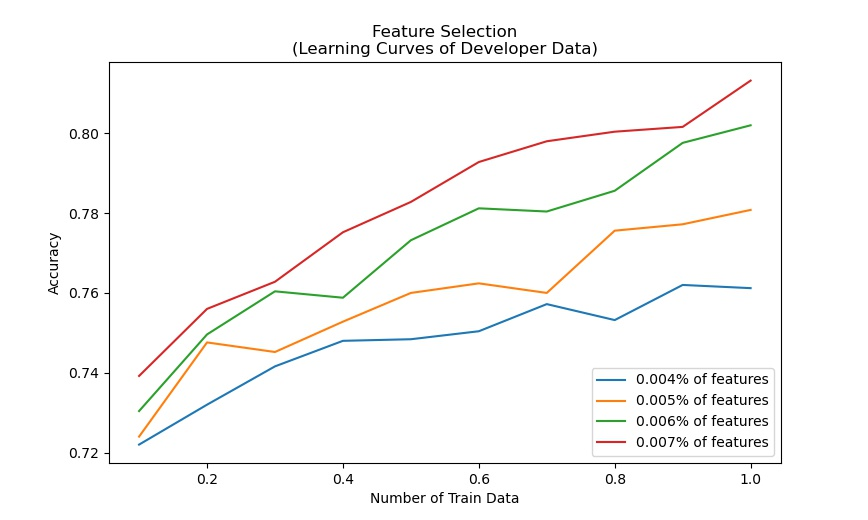
\includegraphics[scale=.55]{images/nb-feature-selection}
    \caption{Feature selection in multinomial Naive Bayes}
    \label{fig:nb-feature-selection}
\end{figure}

\subsection{Καμπύλη Μάθησης}
Για την αποτίμηση του μοντέλου multinomial Naive Bayes, χρησιμοποιούμε ως μετρική την \textbf{ακρίβεια (accuracy)}. Στην Εικόνα \ref{fig:nb-learning-curves}. παρουσιάζονται οι \textbf{καμπύλες μάθησης (learning curves)} από τα δεδομένα εκπαίδευσης και αξιολόγησης. Παρατηρούμε οτι το μοντέλο μας επιτυγχάνει ποσοστά ακρίβειας κοντά στο 81\%.
\begin{figure}[H]
    \centering
    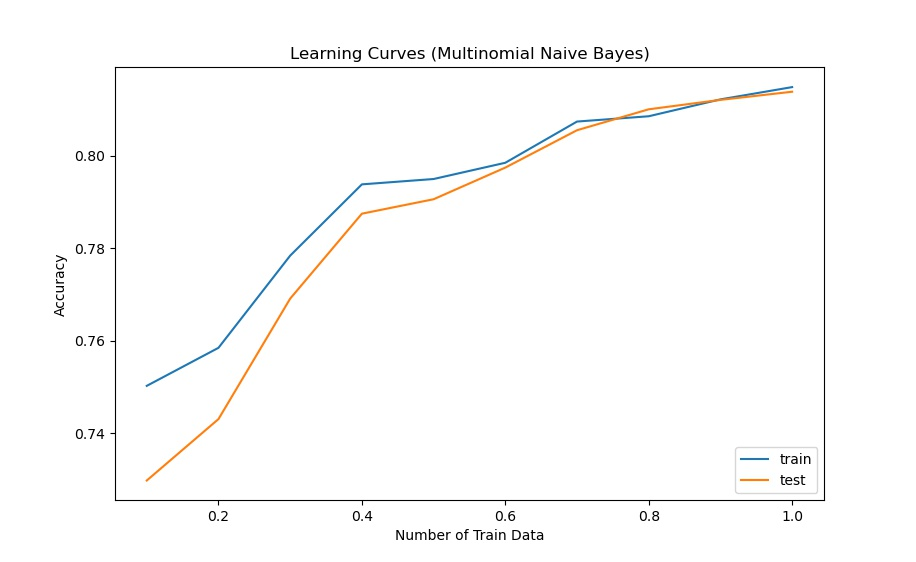
\includegraphics[scale=.5]{images/nb-learning-curve}
    \caption{Multinomial Naive Bayes learning curves}
    \label{fig:nb-learning-curves}
 \end{figure}


\subsection{Καμπύλη Precision-Recall}
Για τον υπολογισμό των μετρικών \textbf{ακρίβεια (precision)} και \textbf{ανάκληση (recall)} έχουμε επιλέξει την χρήση 10 thresholds. Στην Εικόνα \ref{fig:nb-precision-recall} παρατηρούμε ότι καθώς μειώνεται το precision, αυξάνεται το recall με αποτέλεσμα να έχουμε λιγότερα false negatives κατά την κατάταξη. Αντίστοιχα, καθώς μειώνεται το recall αυξάνεται το precision επιτυγχάνοντας λιγότερα false positives.
\begin{figure}[H]
    \centering
    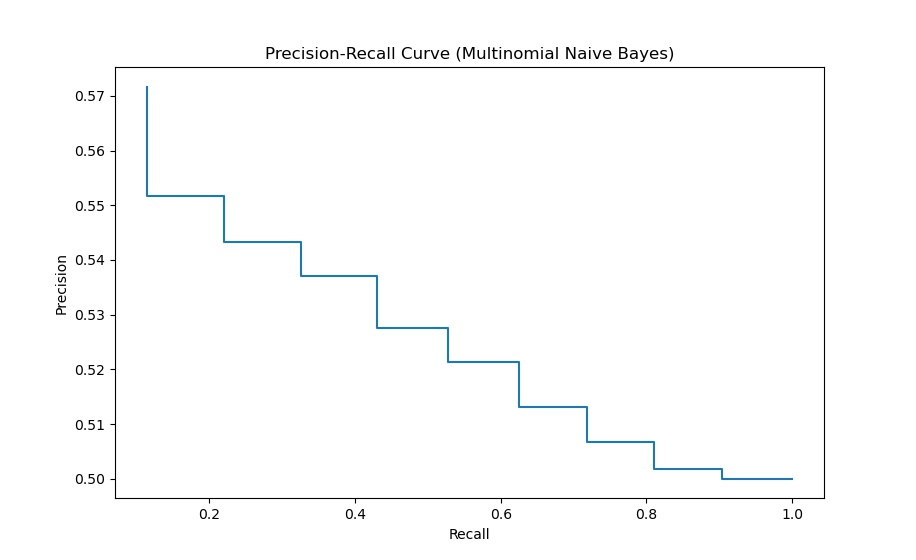
\includegraphics[scale=.5]{images/nb-precision-recall}
    \caption{Multinomial Naive Bayes precision-recall curve}
    \label{fig:nb-precision-recall}
 \end{figure}

\subsection{Καμπύλη F1}
Στην Εικόνα \ref{fig:nb-f1} παρουσιάζεται η τιμή της μετρικής \textbf{f1} για κάθε ένα από τα 10 thresholds που είχαμε επιλέξει για τον υπολογισμό της καμπύλης precision-recall.
\begin{figure}[H]
    \centering
    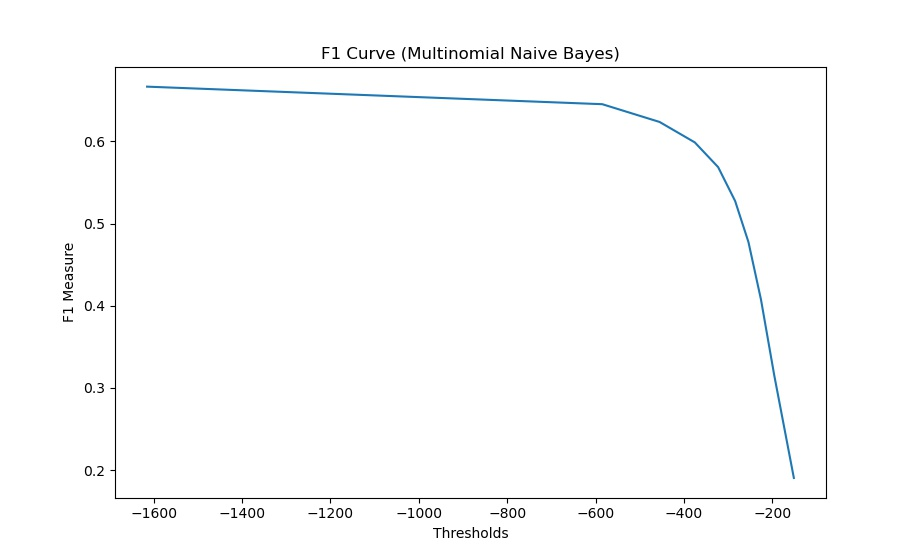
\includegraphics[scale=.5]{images/nb-f1}
    \caption{Multinomial Naive Bayes f1 curve}
    \label{fig:nb-f1}
 \end{figure}

%% -------------------------------------------------------------------------------------
\section{Random Forest με ID3}
Το μοντέλο \textbf{Random Forest} αποτελεί ένα μοντέλο μάθησης συνόλου (ensemble learning). Συγκεκριμένα, δημιουργεί πολλά δένδρα αποφάσεων, όπου κάθε ένα τέτοιο δένδρο, δέχεται ως είσοδο ένα νέο σύνολο δεδομένων, ίδιου μεγέθους και δεδομένα με το αρχικό σύνολο. Xρησιμοποιεί τη τεχνική \textbf{bootstrapping}, δηλαδή για κάθε νέο σύνολο δεδομένων επιλέγει τυχαία κείμενα με επανατοποθέτηση. Μάλιστα, δέχεται ως είσοδο ένα σύνολο επιλεγμένων τυχαία ιδιοτήτων, από το αρχικό υποσύνολο καλύτερων ιδιοτήτων, χωρίς επανατοποθέτηση.\\
Για να προβλέψει την κλάση ενός κειμένου, τα δέντρα αποφάσεων τρέχουν παράλληλα. Κάθε ένα τέτοιο δέντρο παράγει μια απόφαση, δηλαδή την κλάση στόχο που θεωρεί οτι ανήκει το κείμενο. Αυτές οι αποφάσεις συλλέγονται και επιστρέγεται εκείνη που συμφωνεί με την πλειοψηφία.\\\\
Για την υλοποίηση των δέντρα αποφάσεων έχουμε επιλέξει τον ταξινομητή \textbf{ID3}. Η λειτουργία ενός δέντρου αποφάσεων είναι η εξής: 
\begin{itemize}
    \item Βρίσκει την ιδιότητα με το μεγαλύτερο κέρδος πληροφορίας (βλέπε Ενότητα 3). Με αυτό τον τρόπο ελπίζουμε να φτάσουμε στην σωστή ταξινόμηση με όσο το δυνατόν μικρό αριθμό ελέγχων χαρακτηριστικών.
    \item Χωρίζει τα δεδομένα που λαμβάνει ως είσοδο, σε δύο μέρη σύμφωνα με το αν υπάρχει η ιδιότητα ή όχι στα κείμενα.
    \item Επαναλαμβάνει την διαδικασία μεχρι να φτάσει σε τελικούς κόμβους. Γνωρίζουμε οτι βρισκόμαστε σε τελική κατάσταση όταν όλα τα δεδομένα, στον κόμβο προς εξέταη, ανήκουν σε μια από τις δύο κλάσεις, ή όταν δεν έχουμε άλλα χαρακτηριστικά για να ελέγξουμε ή όταν έχουμε φτάσει το μέγιστο βάθος.
\end{itemize}

\subsection{Υπερπαράμετροι}
Για την επιλογή των υπερπαραμέτρων στηριχθήκαμε στη καμπύλη μάθησης από τα δεδομένα επικύρωσης (validation data).\\ 
Πρώτα, με κάποιες τυχαίες δοκιμές αποφασίσαμε ότι o καλύτερος αριθμός από \textbf{ιδιότητες (features)} είναι 100, εκ των οποίων οι 80 θα επιλέγονται τυχαία και θα δίνονται ως είσοδο στο δένδρο.\\
Στη συνέχεια, επιλέξαμε το \textbf{μέγιστο βάθος δέντρου (max depth)}, δοκιμάζοντας τα βάθη 5, 7, 10. Η καλύτερη τιμή accuracy επιτυγχάθηκε με βάθος 10 (την μέγιστη ακρίβεια θα μπορούσαμε να την έχουμε χρησιμοποιώντας το μέγιστο βάθος, πράγμα που απαιτεί αρκετή υπολογιστική ισχυς). Στα βάθη 5 και 7 παρατηρήθηκε το πρόβλημα του περιορισμένου χώρου αναζήτησης καθώς η τιμή της μετρικής accuracy από τα δεδομένα επικύρωσης ήταν χαμηλή.\\
Τέλος, για τον αριθμό των δένδρων που θα παράγονται από τον Random Forest, έγιναν δοκιμές για τις τιμές 10, 30, 50 και 100. Παρατηρήσαμε ότι όσο μεγαλύτερη είναι η τιμή των δένδρων που παράγονται τόσο καλύτερη είναι η τιμή της μετρικής accuracy.

\subsection{Καμπύλη Μάθησης}
Για την αποτίμηση του μοντέλου Random Forest, χρησιμοποιούμε ως μετρική την \textbf{ακρίβεια (accuracy)}. Στην Εικόνα \ref{fig:rf-learning-curves}. παρουσιάζονται οι \textbf{καμπύλες μάθησης (learning curves)} από τα δεδομένα εκπαίδευσης και αξιολόγησης. Παρατηρούμε οτι το μοντέλο μας επιτυγχάνει ποσοστά ακρίβειας κοντά στο 71\%.
\begin{figure}[H]
    \centering
    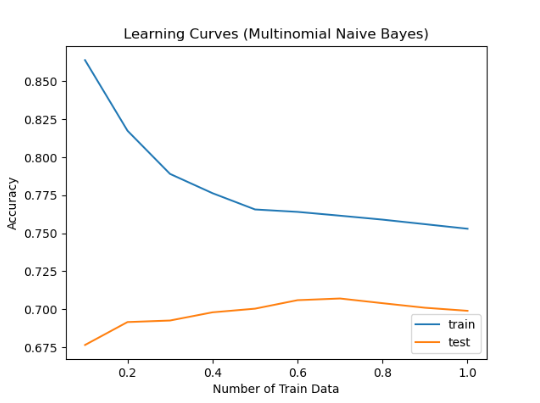
\includegraphics[scale=.8]{images/rf-learning-curve}
    \caption{Random Forest learning curves}
    \label{fig:rf-learning-curves}
 \end{figure}


\subsection{Καμπύλη Precision-Recall}
Για τον υπολογισμό των μετρικών \textbf{ακρίβεια (precision)} και \textbf{ανάκληση (recall)} έχουμε επιλέξει την χρήση 10 thresholds. Στην Εικόνα \ref{fig:rf-precision-recall} παρατηρούμε ότι μεταξύ των σημέιων 0 και 0.2 του οριζόντιου άξονα υπάρχει μια πτώση την μετρικής precision και έπειτα αύξηση. Υποθέτουμε οτι η συμπεριφορά αυτή οφείλεται στο γεγονός ότι υπάρχουν περισσοτερα false positives από true positives. Αντίστοιχα, μεταξύ των τιμών 0.4 και 0.6 του οριζόντιου άξονα παρατηρούμε μια αύξηση της μετρικής precision καθώς η μετρική recall αυξάνεται. Αυτό μπορεί να οφείλεται στο γεγονός ότι τα true positives είναι πολυ περισσοτερα των false positives.
\begin{figure}[H]
    \centering
    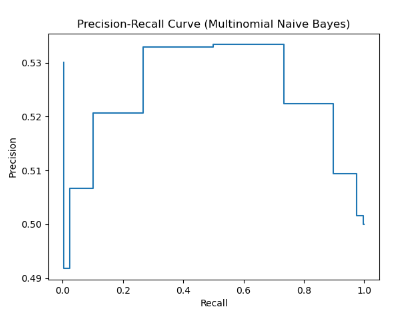
\includegraphics[scale=1]{images/rf-precision-recall}
    \caption{Random Forest precision-recall curve}
    \label{fig:rf-precision-recall}
 \end{figure}

\subsection{Καμπύλη F1}
Στην Εικόνα \ref{fig:rf-f1} παρουσιάζεται η τιμή της μετρικής \textbf{f1} για κάθε ένα από τα 10 thresholds που είχαμε επιλέξει για τον υπολογισμό της καμπύλης precision-recall.
\begin{figure}[H]
    \centering
    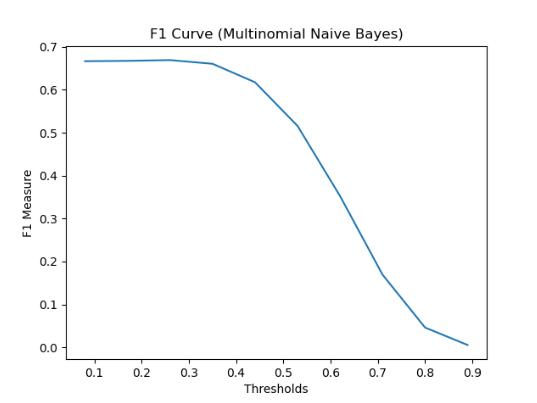
\includegraphics[scale=.8]{images/rf-f1}
    \caption{Random Forest f1 curve}
    \label{fig:rf-f1}
 \end{figure}
 
 \section*{Βιβλιογραφία}
 \begin{enumerate}
     \item C. D. Manning, P. Raghavan, H. Schutze "An Introduction to Information Retrieval"
     \item S. Buttcher, C. L. A. Clarke, G. V.Cormack "Information Retrieval: Implementing and Evaluating Search Engines"
    \item S. Russel, P. Norvig "Artificial Intelligence: A Modern Approach"
    \item T. M. Mitchell "Machine Learning"
 \end{enumerate}
 

\end{document}
